\documentclass{article}
\usepackage[T1]{fontenc}
\usepackage{lmodern}
\usepackage{graphicx}
\usepackage{amsmath,amssymb}
\usepackage[a4paper,margin=2cm]{geometry}
\usepackage[absolute,overlay]{textpos}
\setlength{\TPHorizModule}{1mm}
\setlength{\TPVertModule}{1mm}
\usepackage[indonesian]{babel}
\usepackage{hyperref}
\setlength{\emergencystretch}{2em}
% unit: Halaman 6

\begin{document}

% === Halaman 6 (llm) ===

\section*{A. Cipher Substitusi}

\vspace{50.49mm}

\begin{itemize}
    \item Contoh yang terkenal: \textit{Caesar Cipher}
    \item Tiap huruf alfabet digeser 3 huruf ke kanan
\end{itemize}

\vspace{40mm}

\begin{verbatim}
Plainteks  : A B C D E F G H I J K L M N O P Q R S T U V W X Y Z
Cipherteks : D E F G H I J K L M N O P Q R S T U V W X Y Z A B C
\end{verbatim}

\vspace{56.43mm}

\begin{itemize}
    \item Contoh:
    \begin{itemize}
        \item Plainteks: temui saya di jembatan merah nanti malam
        \item Cipherteks: WHPXL VDBD GL MHPEDWDQ PHUDK QDQWL PDODP
    \end{itemize}
\end{itemize}

% deskripsi: Diagram ilustrasi pergeseran huruf alfabet dalam Caesar Cipher, menunjukkan pemetaan huruf A menjadi D, B menjadi E, dan seterusnya.
% bbox normalisasi: [0.5400, 0.2000, 0.9700, 0.3700]
\begin{textblock*}{90.30mm}(113.40mm,59.40mm)
\noindent
\includegraphics[width=90.30mm,height=50.49mm]{../../images/llm/page_006_img_01.png}%
\end{textblock*}

% deskripsi: Potret patung Julius Caesar, tokoh yang mempopulerkan Caesar Cipher.
% bbox normalisasi: [0.7700, 0.5500, 0.9400, 0.9700]
\begin{textblock*}{35.70mm}(161.70mm,163.35mm)
\noindent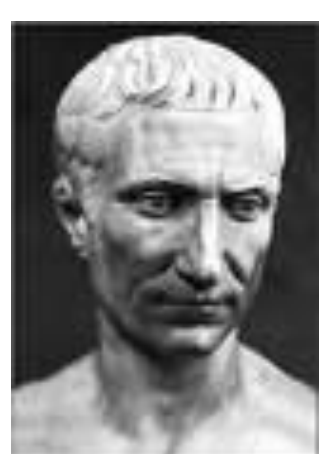
\includegraphics[width=35.70mm,height=124.74mm]{../../images/llm/page_006_img_02.png}%
\end{textblock*}

% deskripsi: Ilustrasi lukisan bertema Romawi kuno.
% bbox normalisasi: [0.0000, 0.8100, 0.1400, 1.0000]
\begin{textblock*}{29.40mm}(0.00mm,240.57mm)
\noindent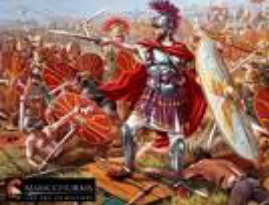
\includegraphics[width=29.40mm,height=56.43mm]{../../images/llm/page_006_img_03.png}%
\end{textblock*}

\end{document}
